% !TeX spellcheck = en_US
\section{Digital Transformation}
\subsection{Basics}
\begin{compactitem}
	\item Digital Transformation = Fundamental and disruptive change how we organize us and produce goods and services
	\item Main key is to collect and digitalise phenomena (data)
	\item Our culture (mainly private companies...) collects a comprehensive data-„picture“ about the world. That’s the logic continuation of cartography and description in books, photos etc.
	\item Large amounts of data is commodity for digital products (big data	\& analytics)
\end{compactitem}

\subsection{Exponential growth of technology}
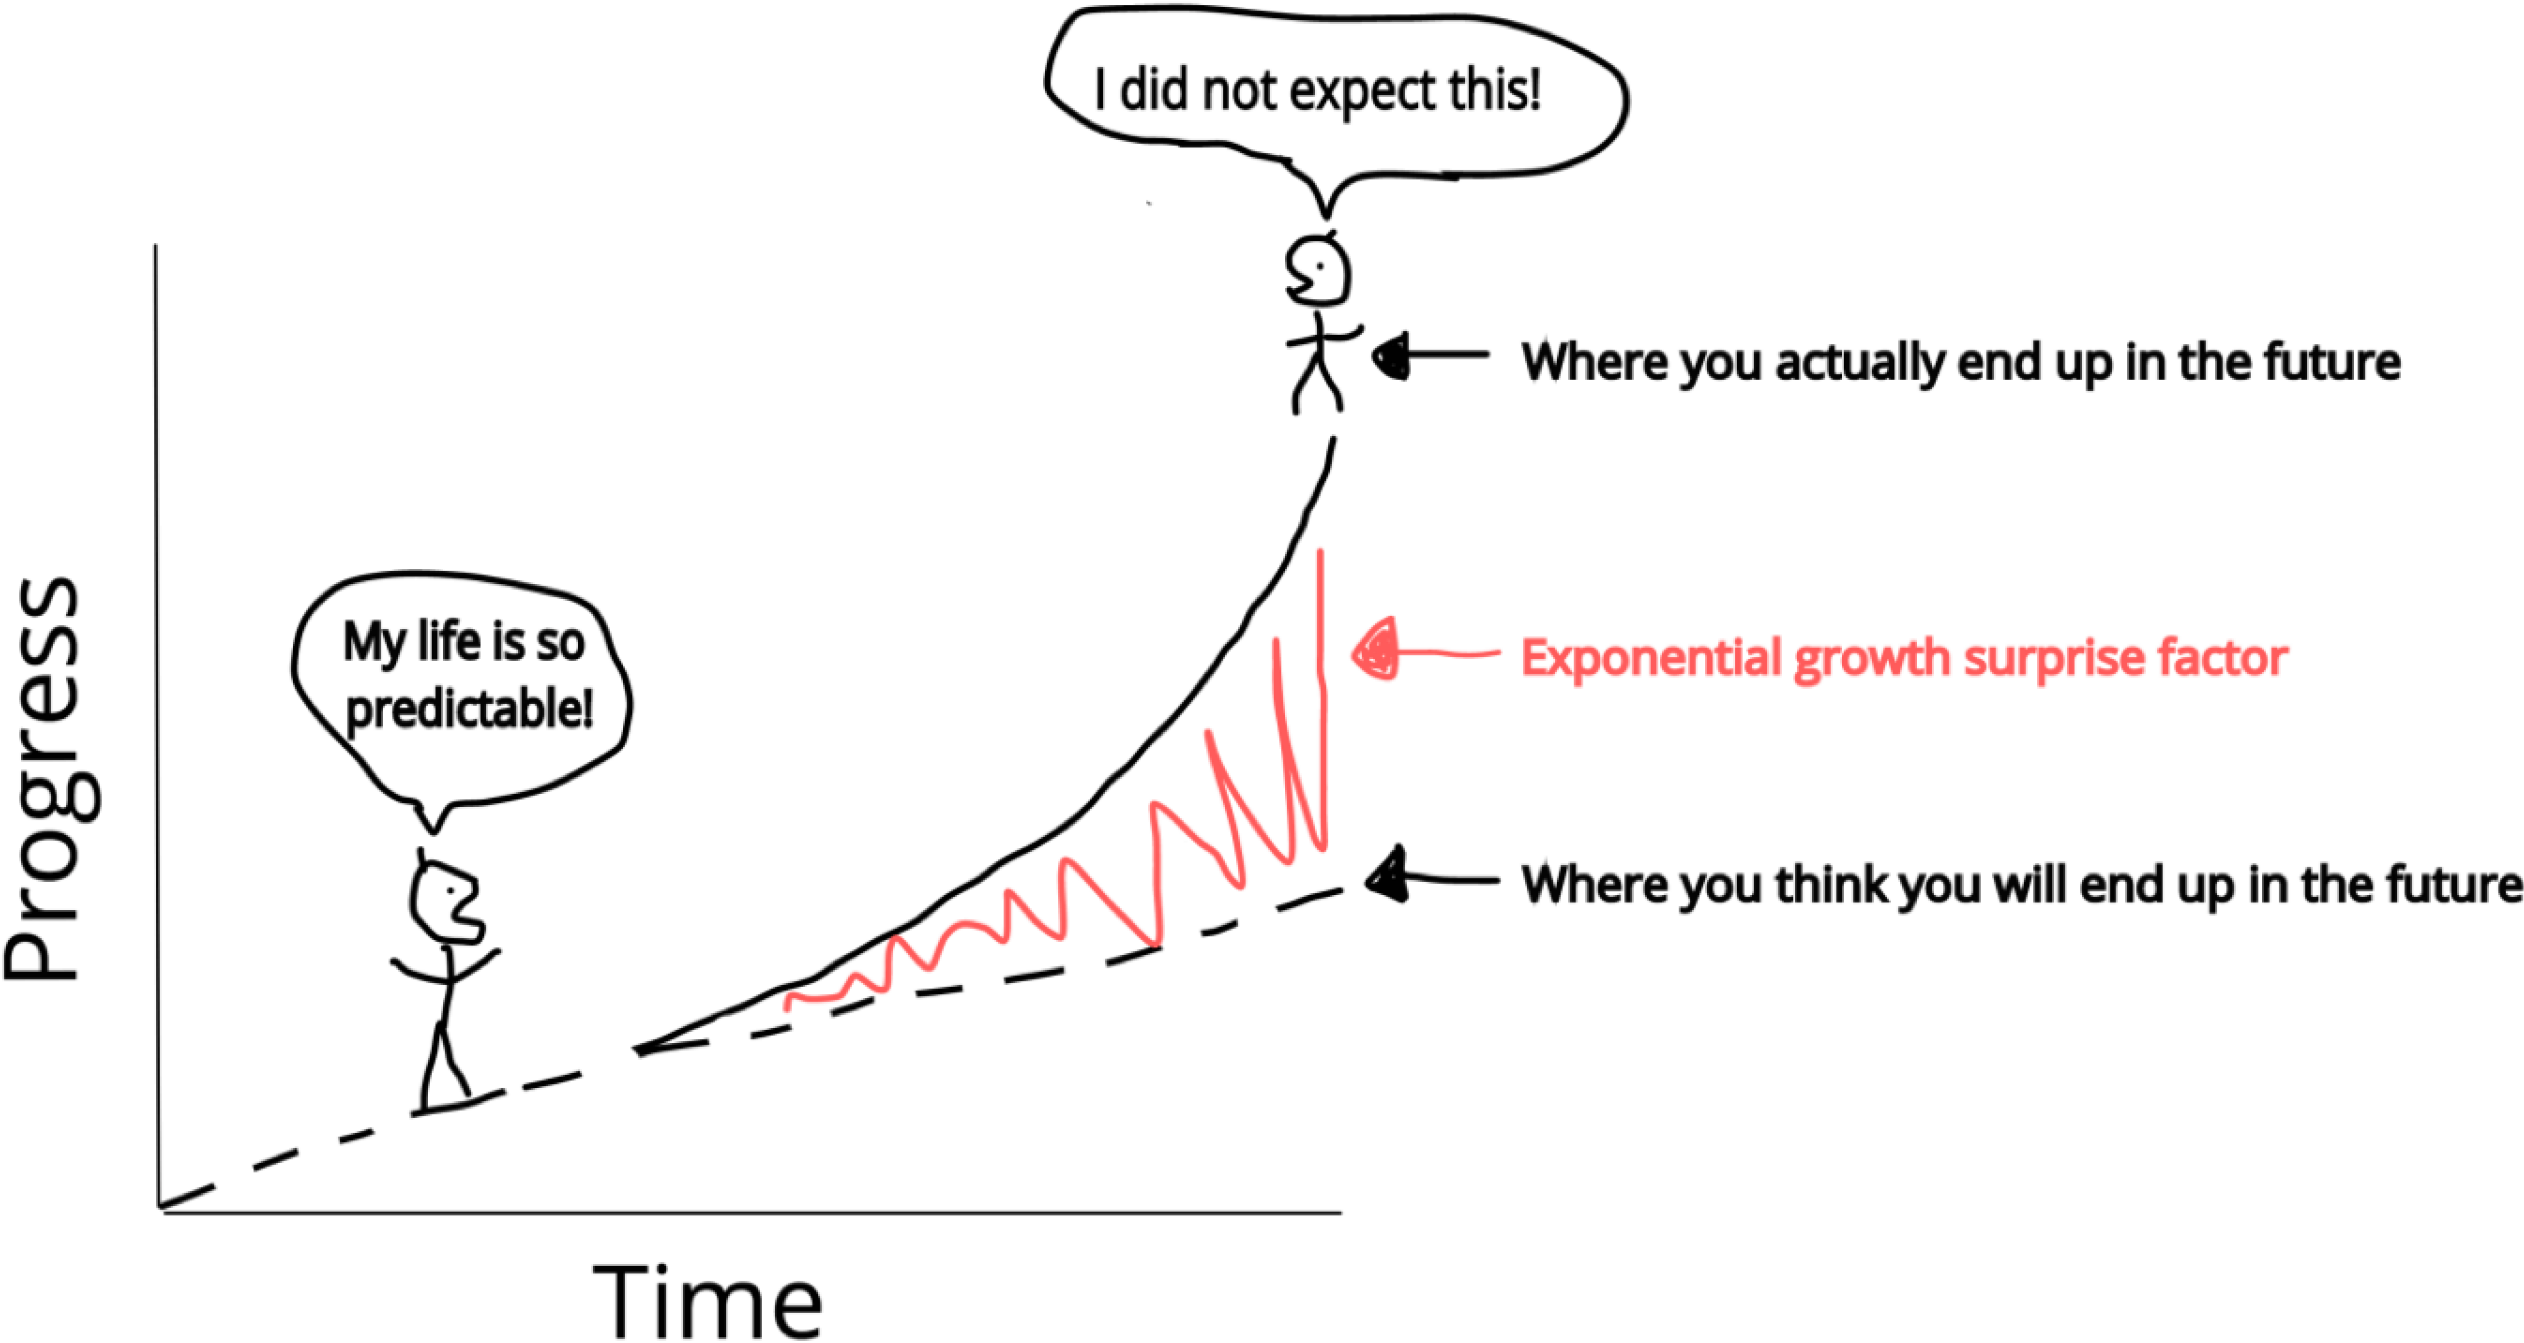
\includegraphics[width=1\linewidth]{images/exponential_growth_of_technology}

%\subsection{Moore's law and it's consequences}
%\begin{compactitem}
%	\item Moore’s Law = Doubling the digital calculation power nearly every second year (results in an exponential curve) with sinking costs. Results in the zero marginal costs.
%	\item Moore’s Law is still valid but actual technology (2018) is coming the next years to its limit.
%	\item BUT - new technologies - ie. quantum computers are for specific mathematic problems already today in their experimental state dramatically faster.
%\end{compactitem}

\subsection{Digital business models}
\begin{compactitem}
	\item It is the backbone of any company!
	\item Digitalization has for organizations many advantages, ie. a better connection to the customers, higher efficiency and the chance to develop new products and services.
	\item But Digital Business works particularly on different economic principles.	Traditional experience sometimes doesn’t work!
	\item „You can’t walk in sneakers to the moon!“. Sometimes you have to change the method!
	\item „Edison didn’t invented the bulb by evolving the gas light...“ Do something different!
\end{compactitem}

\subsection{New culture}
\begin{compactitem}
	\item Fast is the new big!
	\item Fast = more  \& constant communication
	\item Shorter development times = shorter time to market = less risk
	\item Shorter development times = culture of fail fast \& learn faster!
	\item Be transparent \& congruent! Also for your costumers! (Data Protection...)
\end{compactitem}

\subsection{Big data, AI and Machine Learning}
\begin{compactitem}
	\item The term "big data" stands for a large volume of data from a variety of sources which is rapidly collected, stored and made available for indefinite purposes for an indefinite period of time for analysis and evaluation.
	\item This intensive processing is now possible due to technological developments which make it much cheaper and faster to store and evaluate huge data volumes.
	\item New methods and technologies facilitate the analysis and linking of very large amounts of data with ease. Algorithms are applied to large databases in order to recognize new patterns, similarities, relationships or discrepancies.
	\item Free software (i.e. Torch or Sensorflow) and cheap hardware (Nvidia) enables to develop cheap and fast analysis-tools/products. Since 6 month more \& more cheap software and tool are on the market (.e. qnamaker.ai, bots etc.)
\end{compactitem}

\subsection{Data intelligence}
\begin{compactitem}
	\item Data intelligence refers to the analysis of data in a way that allows the	data to be used by a company to expand its services or investments.
	\item Companies can also use data intelligence to evaluate internal data. This enables them to analyze their own activities and activities of their staff so they can make better decisions in the future. In very general terms, data intelligence should provide useful conclusions for the future from the analysis of current data. When processing personal data, companies must always observe data protection regulations.
	\item Example: play with your website-design and use Google Analytics to measure the effects. Repeat.
\end{compactitem}

\subsection{The four V of big data}
Big data can basically be defined through four features. They are known as the four „V“s:
\begin{compactitem}
	\item Big data involves large amounts of data (VOLUME) that are...
	\item ...processed at high speed (VELOCITY).
	\item The third V is the VARIETY of data. Big data permits new options of combining data from different sources that previously had no connection. Pattern recognition!
	\item Finally, data analysis creates added value (VALUE).
\end{compactitem}

\subsection{Datability}
\begin{compactitem}
	\item Datability means the responsible and sustainable handling of data (or data media).
	\item The word was created to express the fact that data processers also have an important responsibility towards systems, users and the future. The term has triggered a value discussion and a drive to measure responsibility in the creation of IT systems as well as corporate responsibility. It will certainly also have an effect on future legislative projects.
\end{compactitem}

\subsection{Legal aspects of digitalization of company processes}
Regulations about:
\begin{compactitem}
	\item Handling of digital invoices (ElDI-V)
	\item Digital data archives (GeBüV) \& Art. 958f Code of Obligations (OR)
	\item Personal data protection (DSG/GDPR)
	\item Duties to inform customers (UWG)
	\item Intellectual properties (URG)
	\item Unfair competition (UWG)
	\item ...
\end{compactitem}

\subsection{Is law a limiting factor?}
Sometimes yes.
\begin{compactitem}
	\item You have to address \& answer legal questions very early in projects.
	\item For some questions law hasn’t (yet) a clear answer: smart contracts, blockchain, virtual companies, AI etc. Then you have to find a „workaround“ or have to take the risk.
	\item But often for competitor abroad! Our law is quit liberal and mostly not strict. That’s a huge advantage!
\end{compactitem}
